% !TeX program = xelatex
% !TeX options = -shell-escape
% !TEX encoding = UTF-8

% --------------------------------------------------------------
% This is all preamble stuff that you don't have to worry about.
% Head down to where it says "Start here"
% --------------------------------------------------------------

\documentclass[12pt]{article}
\usepackage[margin=2cm]{geometry} % 頁面邊距設置
\usepackage{amsmath,amssymb,amsthm} % 數學相關套件
\usepackage{graphicx} % 圖形插入
\usepackage{booktabs} % 表格線條
\usepackage[AutoFakeBold,AutoFakeSlant]{xeCJK} % 中文支援
\usepackage{fancyhdr} % 頁首頁尾設置
\usepackage{xcolor,changepage,mdframed} % 顏色與框線相關
\usepackage{titlesec} % 標題格式
\usepackage{setspace} % 行距
\usepackage{minted} % 程式碼高亮（需安裝 Python 套件 pygments）
\usepackage{ulem}
\usepackage[shortlabels]{enumitem} % 列表格式
\usepackage[colorlinks=true,linkcolor=black,urlcolor=blue,citecolor=blue]{hyperref}
% 超連結
\graphicspath{{images}}

% 字體設定 (xeCJK)
\setCJKmainfont{黑體-繁}
\setCJKmonofont{Noto Sans Mono CJK TC}

% 頁首/頁尾設定 (fancyhdr)
\pagestyle{fancy}
\fancyhead[L]{NASA Homework 9} % 可以用 \leftmark 取代
\fancyhead[R]{B13901011 吳亞倫}
\fancyfoot[C]{\thepage}
\renewcommand{\headrulewidth}{0.4pt}
\renewcommand{\footrulewidth}{0pt}
\setlength{\headheight}{15pt}

% tex-fmt: off
\newtheorem*{theorem}{Theorem}
\newenvironment{lemma}[2][Lemma]{\begin{trivlist}
\item[\hskip \labelsep {\bfseries #1}\hskip \labelsep {\bfseries #2.}]}{\end{trivlist}}
\newenvironment{exercise}[2][Exercise]{\begin{trivlist}
\item[\hskip \labelsep {\bfseries #1}\hskip \labelsep {\bfseries #2.}]}{\end{trivlist}}
\newenvironment{problem}[2][Problem]{\begin{trivlist}
\item[\hskip \labelsep {\bfseries #1}\hskip \labelsep {\bfseries #2}]}{\end{trivlist}}
\newenvironment{question}[2][Question]{\begin{trivlist}
\item[\hskip \labelsep {\bfseries #1}\hskip \labelsep {\bfseries #2.}]}{\end{trivlist}}
\newenvironment{corollary}[2][Corollary]{\begin{trivlist}
\item[\hskip \labelsep {\bfseries #1}\hskip \labelsep {\bfseries #2.}]}{\end{trivlist}}
\newenvironment{solution}{\begin{proof}[Solution]}{\end{proof}}
\newenvironment{answer}{\begin{proof}[Ans]}{\end{proof}}
\renewcommand{\thesubsubsection}{\thesubsection. (\alph{subsubsection})}

% 樣式設定

\setminted{frame=lines, linenos, framesep=2mm, breaklines=true, breakanywhere=true, autogobble=true}

% 自訂框線環境
\newmdenv[
  linewidth=2pt, linecolor=gray, backgroundcolor=gray!10,
  topline=false, bottomline=false, rightline=false,
  skipabove=10pt, skipbelow=10pt, innerleftmargin=10pt,
  innerrightmargin=0pt, innertopmargin=5pt, innerbottommargin=5pt
]{myquote}

\newenvironment{mycolorbox}[1][gray]{
  \renewmdenv[
    linewidth=2pt, linecolor=#1, backgroundcolor=#1!10,
    topline=false, bottomline=false, rightline=false,
    skipabove=10pt, skipbelow=10pt, innerleftmargin=10pt,
    innerrightmargin=0pt, innertopmargin=5pt, innerbottommargin=5pt
  ]{myquote}
  \begin{myquote}
}{\end{myquote}}

\linespread{1.1}
% \usemintedstyle{xcode}
\AtBeginEnvironment{minted}{\vspace{-10pt}} % 可根據需求調整間距數值
\setminted{breaklines=true, breakanywhere=true, autogobble=true}

% tex-fmt: on
\begin{document}
\thispagestyle{fancy}

%------------------------------------------------------------
%                         Start here
% -----------------------------------------------------------

\begin{center}
  {\large \bfseries Network Administration / System Administration} \\
  \vspace{1em}
  {\Large \bfseries Homework 9} \\
\end{center}

\vspace{2em}

\begin{tabular}{@{}l l}
  \textbf{Student:} & 吳亞倫 \\
  \textbf{ID:} & B13901011  \\
  \textbf{Department:} & 電機工程學系
\end{tabular}
\bigskip

\begin{mycolorbox}[cyan]
  \textbf{Discussion Partners:}
  \begin{itemize}
    \item Classmates：賴泓安、鄭竣陽、喻慈恩
      \vspace{0.5em}
  \end{itemize}
\end{mycolorbox}

% Problem 1
\section{系統環境與 NFS 基礎安裝}

\begin{mycolorbox}[teal]
  \textbf{Reference:}
  \footnotesize
  \begin{itemize}
    \item \href{https://caloskao.org/using-netplan-to-configure-ubuntu-nic/}{使用 Netplan 進行 Ubuntu 的網路卡設定}
    \item \href{https://documentation.ubuntu.com/server/how-to/networking/install-nfs/index.html}{Network File System (NFS)}
  \end{itemize}
\end{mycolorbox}
\setcounter{subsection}{-1}
\subsection{Setup}
\begin{enumerate}
  \item 首先，我啟動三台虛擬機之後，以 VNC 連線上去，並且以 lab 的方法啟動 \texttt{ens3} 與 \texttt{ens4} 兩個網路介面卡。
  \item 虛擬機中沒有 \texttt{dhclient}，所以我建立 \texttt{/etc/netplan/nasa.yaml} 來手動設定 \texttt{ens3} 和 \texttt{ens4} 的IP 位址。
  \begin{minted}{yaml}
    network:
      ethernets:
          ens3:
              addresses: [10.0.2.15/24]
              nameservers:
                  addresses: [8.8.8.8]
              routes:
              -   to: default
                  via: 10.0.2.2
          ens4:
              addresses: [192.168.128.73/24]
      version: 2
  \end{minted}
  \item 將其他的 yaml 檔案移除，並且執行 \texttt{sudo netplan apply} 來套用設定。
  \item 設定完成後，三台虛擬機的 IP 位址分別為：
  \begin{itemize}
    \item \texttt{hpc1}: \texttt{192.168.128.71}
    \item \texttt{hpc2}: \texttt{192.168.128.72}
    \item \texttt{nfs-server}: \texttt{192.168.128.73}
  \end{itemize}
\end{enumerate}

\subsection{NFS Server 端設定}
\begin{enumerate}
  \item 我按照 lab 的指示，安裝 NFS Server，並編輯 \texttt{/etc/exports} 檔案，加入以下內容：
  \begin{minted}{bash}
    /srv/nfs-share 192.168.128.0/24(rw,sync,fsid=0,crossmnt,no_subtree_check) 
  \end{minted}
  \item 更改資料夾權限：
  \begin{minted}{bash}
    sudo mkdir -p /srv/nfs-share
    sudo chown 1000:1000 /srv/nfs-share/
    sudo chmod 755 /srv/nfs-share
  \end{minted}
  \item 套用設定並且啟動 NFS Server：
  \begin{minted}{bash}
    sudo exportfs -arv 
    sudo systemctl enable --now nfs-server
    sudo systemctl restart nfs-server
  \end{minted}
  \begin{figure}[H]
    \centering
    
\includegraphics[width=0.9\textwidth]{1-1.png}
    \caption{nfs-server 的 NFS 服務確認 }
    \label{fig:1-1}
  \end{figure}
\end{enumerate}

\subsection{Client 端掛載}
\begin{enumerate}
  \item 在 \texttt{hpc1} 與 \texttt{hpc2} 上安裝 NFS Client
  \item 用 lab 的方法掛載 NFS Server 的資料夾：
  \begin{minted}{bash}
    sudo mkdir -p /mnt/nfs-share
    sudo mount -t nfs 192.168.128.73:/srv/nfs-share /mnt/nfs-share
  \end{minted}
  \item 確認掛載成功：
  \begin{figure}[H]
    \centering
    
\includegraphics[width=\textwidth]{1-2-1.png}
    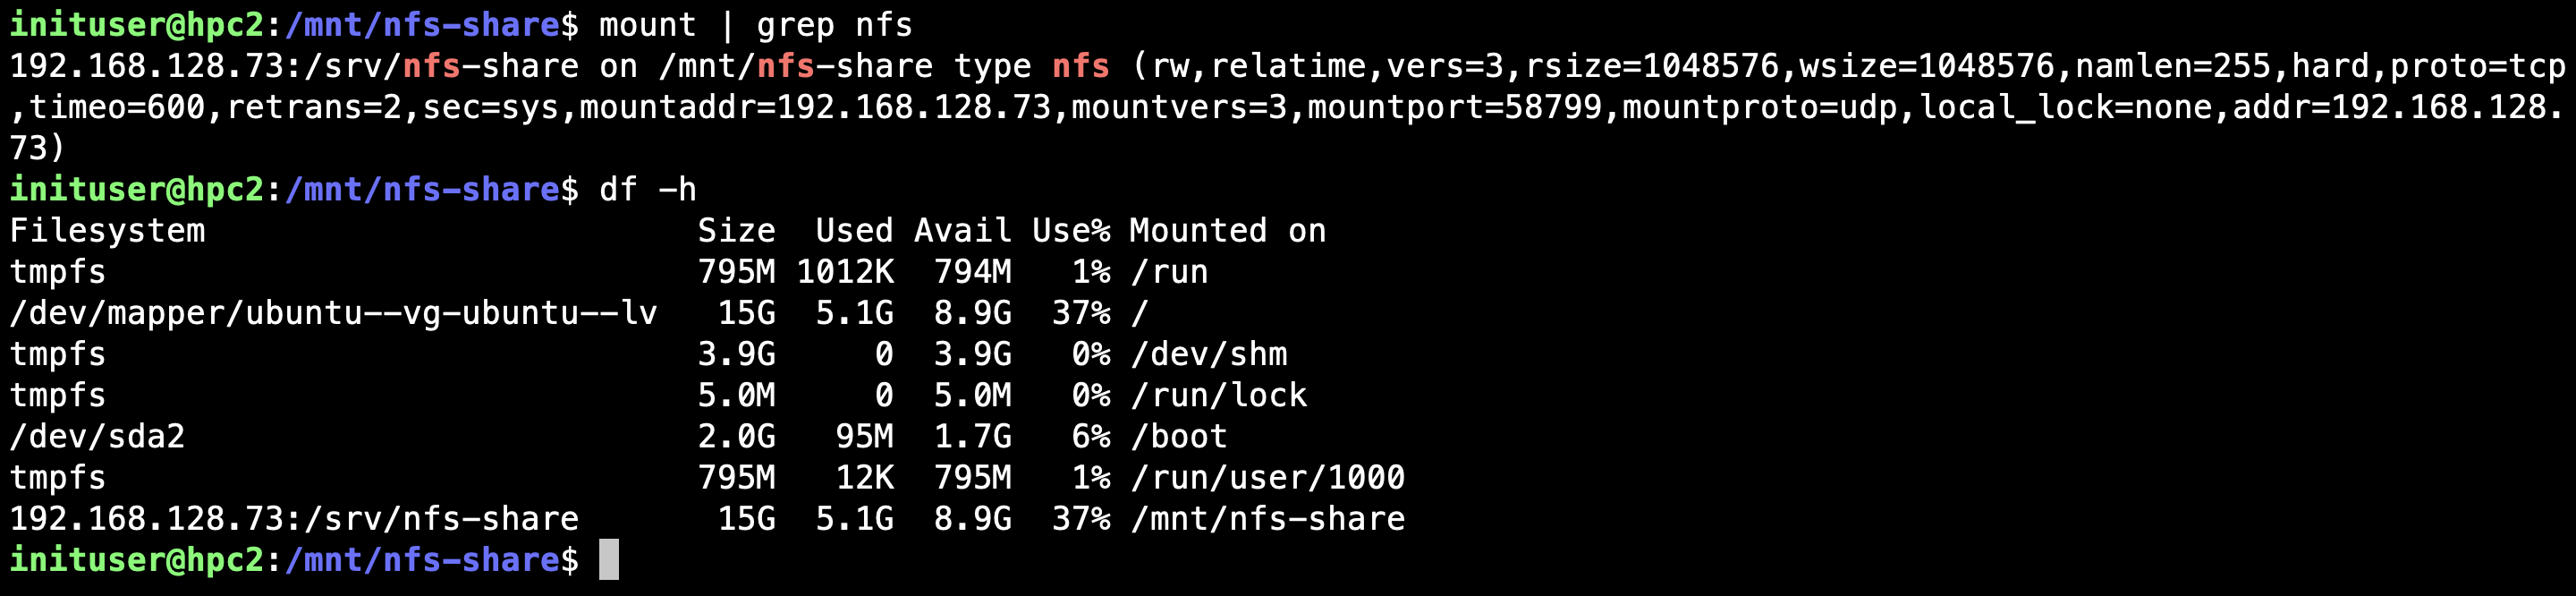
\includegraphics[width=\textwidth]{1-2-2.png}
    \caption{hpc1 與 hpc2 的 NFS 掛載確認 }
    \label{fig:1-2}
  \end{figure}
  \item 完成後，我依序建立了 \texttt{from\_hpc1.txt} 與 \texttt{from\_hpc2.txt} 兩個檔案，並且成功從兩台 Client 端和 NFS Server 端互相讀、寫檔案。
  \begin{figure}[H]
    \centering
    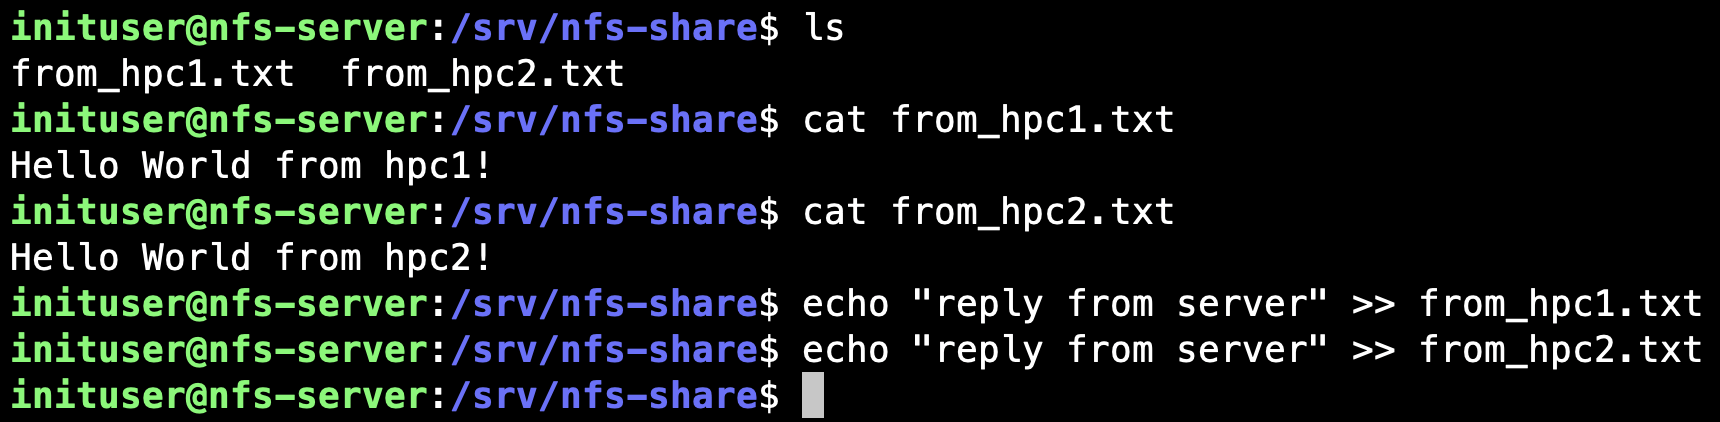
\includegraphics[width=\textwidth]{1-2-3.png}
    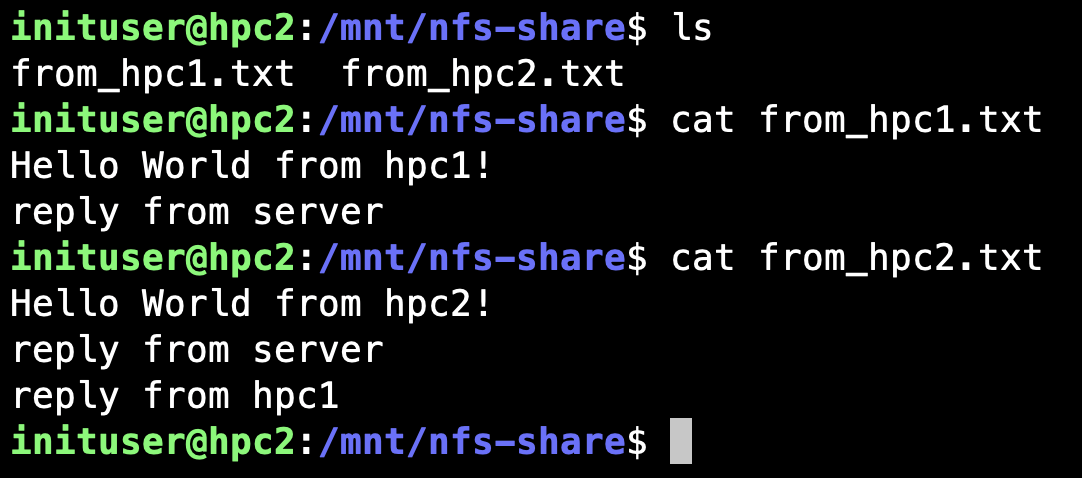
\includegraphics[height=3.19cm]{1-2-4.png}
    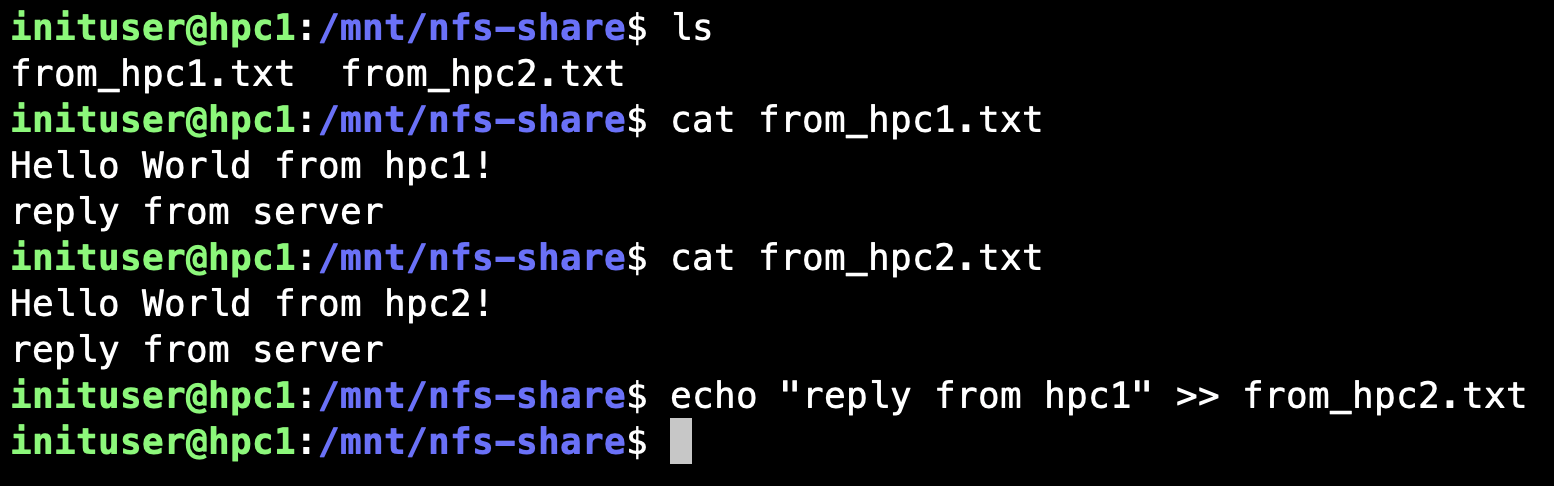
\includegraphics[height=3.19cm]{1-2-5.png}
    \caption{server、hpc1 與 hpc2 的檔案互相讀寫}
    \label{fig:1-3}
  \end{figure}
\end{enumerate}


\clearpage
% Problem 2
\section{多使用者帳號與權限控管}

\begin{mycolorbox}[teal]
  \textbf{Reference:}
  \footnotesize
  \begin{itemize}
    \item \href{https://docs.google.com/presentation/d/1QOBSuBnh2F55daXRpcfpHbN-fNiUS3Hz2edsyFqzFQQ/edit?usp=sharing}{Lab 9 簡報}
    \item Homework 8
    \item \href{https://linux.vbird.org/somepaper/20050817-ldap-1.pdf}{LDAP 入門}
    \item \href{https://www.baeldung.com/linux/ubuntu-ldap-client}{Configuring Ubuntu as an LDAP Client}
  \end{itemize}
\end{mycolorbox}

\subsection{LDAP 與 NFS}
\begin{enumerate}
  \item 建立 \texttt{astro} 的資料夾：
  \begin{minted}{bash}
    sudo mkdir /srv/nfs-share/astro1_dir
    sudo mkdir /srv/nfs-share/astro2_dir
    sudo mkdir /srv/nfs-share/astro3_dir
  \end{minted}
  \item 我在 \texttt{nfs-server} 上安裝 ldap 伺服器套件：
  \begin{minted}{bash}
    sudo apt install slapd ldap-utils
  \end{minted}
  \item 用 \texttt{slappasswd} 產生密碼。
  \item 參考 lab9，我創立 \texttt{setup.ldif} 檔案，並且加入以下內容：
  \begin{minted}{ldif}
    dn: olcDatabase={1}mdb,cn=config
    changetype: modify
    replace: olcSuffix
    olcSuffix: dc=nasa,dc=csie,dc=ntu

    dn: olcDatabase={1}mdb,cn=config
    changetype: modify
    replace: olcRootDN
    olcRootDN: cn=admin,dc=nasa,dc=csie,dc=ntu

    dn: olcDatabase={1}mdb,cn=config
    changetype: modify
    replace: olcRootPW
    olcRootPW:{SSHA}LZBdH0PETNbAcD6P0cGxVjS9XR2pVNfy
  \end{minted}
  並用 \texttt{ldapmodify -Y EXTERNAL -H ldapi:/// -f rootdn.ldif} 套用設定。
  \clearpage
  \item 建立 \texttt{base.ldif} 檔案，並加入以下內容：
  \begin{minted}{ldif}
    dn: dc=nasa,dc=csie,dc=ntu
    dc: nasa
    objectClass: top
    objectClass: domain

    dn: cn=admin,dc=nasa,dc=csie,dc=ntu
    cn: admin
    objectClass: organizationalRole
    description: admin account

    dn: ou=people,dc=nasa,dc=csie,dc=ntu
    ou: people
    objectClass: organizationalUnit

    dn: ou=group,dc=nasa,dc=csie,dc=ntu
    ou: group
    objectClass: organizationalUnit
  \end{minted}
  並用 \texttt{ldapadd -x -D cn=admin,dc=nasa,dc=csie,dc=ntu -W -f base.ldif} 套用設定。
  \item 建立 \texttt{user.ldif} 檔案，並加入以下內容：
  \begin{minted}{ldif}
    dn: cn=astro1,ou=group,dc=nasa,dc=csie,dc=ntu
    objectClass: posixGroup
    cn: astro1
    gidNumber: 1001

    dn: cn=astro2,ou=group,dc=nasa,dc=csie,dc=ntu
    objectClass: posixGroup
    cn: astro2
    gidNumber: 1002

    dn: cn=astro3,ou=group,dc=nasa,dc=csie,dc=ntu
    objectClass: posixGroup
    cn: astro3
    gidNumber: 1003

    dn: uid=astro1,ou=people,dc=nasa,dc=csie,dc=ntu
    objectClass: inetOrgPerson
    objectClass: posixAccount
    objectClass: shadowAccount
    cn: astro1
    sn: astro1
    uid: astro1
    uidNumber: 1001
    gidNumber: 1001
    homeDirectory: /mnt/nfs-share/astro1_dir
    loginShell: /bin/bash

    dn: uid=astro2,ou=people,dc=nasa,dc=csie,dc=ntu
    objectClass: inetOrgPerson
    objectClass: posixAccount
    objectClass: shadowAccount
    cn: astro2
    sn: astro2
    uid: astro2
    uidNumber: 1002
    gidNumber: 1002
    homeDirectory: /mnt/nfs-share/astro2_dir
    loginShell: /bin/bash

    dn: uid=astro3,ou=people,dc=nasa,dc=csie,dc=ntu
    objectClass: inetOrgPerson
    objectClass: posixAccount
    objectClass: shadowAccount
    cn: astro3
    sn: astro3
    uid: astro3
    uidNumber: 1003
    gidNumber: 1003
    homeDirectory: /mnt/nfs-share/astro3_dir
    loginShell: /bin/bash
  \end{minted}
  並用 \texttt{ldapadd -x -D cn=admin,dc=nasa,dc=csie,dc=ntu -W -f user.ldif} 套用設定。
  \item 使用以下指令為 \texttt{astro1}、\texttt{astro2} 與 \texttt{astro3} 三個使用者設定密碼：
  \begin{minted}{bash}
    ldappasswd -x -D "cn=admin,dc=nasa,dc=csie,dc=ntu" -W \
      -S "uid=astro1,ou=people,dc=nasa,dc=csie,dc=ntu"
    ldappasswd -x -D "cn=admin,dc=nasa,dc=csie,dc=ntu" -W \
      -S "uid=astro2,ou=people,dc=nasa,dc=csie,dc=ntu"
    ldappasswd -x -D "cn=admin,dc=nasa,dc=csie,dc=ntu" -W \
      -S "uid=astro3,ou=people,dc=nasa,dc=csie,dc=ntu"
  \end{minted}
  \item 在 \texttt{hpc1} 與 \texttt{hpc2} 上安裝 ldap client 套件：
  \begin{minted}{bash}
    sudo apt update && sudo apt install libnss-ldap libpam-ldap ldap-utils nscd
  \end{minted}
  \item 安裝時，會需要填寫以下設定：
  \begin{itemize}
    \item \texttt{ldap server: ldap://192.168.128.73}
    \item \texttt{base: dc=nasa,dc=csie,dc=ntu}
    \item \texttt{ldap version: 3}
    \item \texttt{Make local root Database admin: No}
    \item \texttt{Does the LDAP database require login: No}
  \end{itemize}
  \item 編輯 \texttt{/etc/nsswitch.conf}，加入以下內容：
  \begin{minted}{bash}
    passwd: files systemd ldap
    group: files systemd ldap
    shadow: files systemd ldap
  \end{minted}
  \item 編輯 \texttt{/etc/ldap/ldap.conf}，加入以下內容：
  \begin{minted}{bash}
    BASE    dc=nasa,dc=csie,dc=ntu
    URI     ldap://192.168.128.73
  \end{minted}
  \item 重啟 \texttt{nscd} 和 \texttt{nslcd} 服務：
  \begin{minted}{bash}
    sudo systemctl restart nscd
    sudo systemctl restart nslcd
  \end{minted}
  \item 以下為結果確認：
\begin{figure}[H]
  \centering
  
\includegraphics[width=0.49\textwidth]{2-1-1.png}
  
\includegraphics[width=0.49\textwidth]{2-1-2.png}
  
\includegraphics[width=0.49\textwidth]{2-1-3.png}
  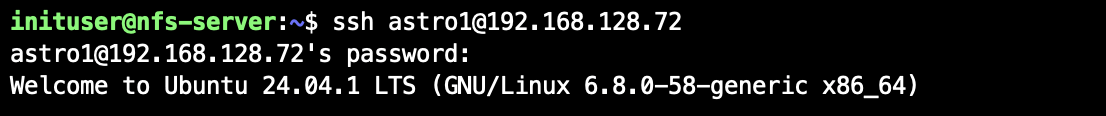
\includegraphics[width=0.49\textwidth]{2-1-6.png}
  
\includegraphics[width=0.49\textwidth]{2-1-4.png}
  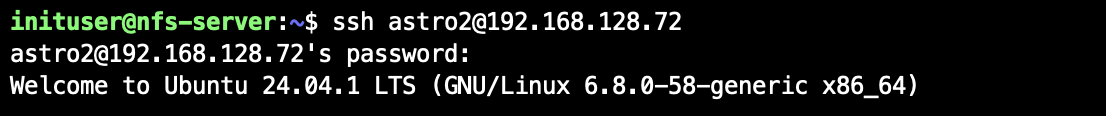
\includegraphics[width=0.49\textwidth]{2-1-7.png}
  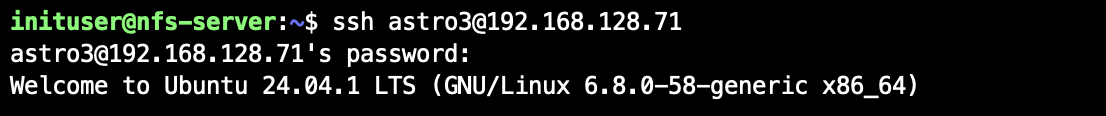
\includegraphics[width=0.49\textwidth]{2-1-5.png}
  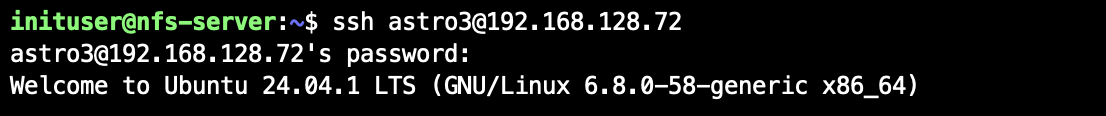
\includegraphics[width=0.49\textwidth]{2-1-8.png}
  \caption{hpc1 與 hpc2 的使用者確認 }
  \label{fig:2-1}
\end{figure}
\end{enumerate}

\subsection{就算是 root 又怎樣？！}
\begin{enumerate}
  \item 在 server 上，我使用以下指令修改資料夾權限：
  \begin{minted}{bash}
    sudo chown 1001:1001 /srv/nfs-share/astro1_dir
    sudo chown 1002:1002 /srv/nfs-share/astro2_dir
    sudo chown 1003:1003 /srv/nfs-share/astro3_dir

    sudo chmod 700 /srv/nfs-share/astro1_dir
    sudo chmod 700 /srv/nfs-share/astro2_dir
    sudo chmod 700 /srv/nfs-share/astro3_dir
  \end{minted}
  \item 修改 \texttt{/etc/exports} 檔案，修改以下內容：
  \begin{minted}{bash}
    /srv/nfs-share      192.168.128.0/24(rw,sync,fsid=0,crossmnt,no_subtree_check,root_squash)
  \end{minted}
  \item 套用設定並且重啟 NFS Server：
  \begin{minted}{bash}
    sudo exportfs -arv 
    sudo systemctl restart nfs-server
  \end{minted}
  \item 我使用以下指令確認權限：
  \begin{minted}{bash}
    ls -l /srv/nfs-share
  \end{minted}
  以下為結果確認：
  \begin{figure}[H]
    \centering
    
\includegraphics[width=0.9\textwidth]{2-2.png}
    \caption{server 的權限確認}
    \label{fig:2-2}
  \end{figure}
  \item 以下為我在 \texttt{hpc1} 上，分別以 \texttt{astro1}、\texttt{astro2} 與 \texttt{root} 帳號嘗試進入 \texttt{astro1\_dir} 的結果：
  \begin{figure}[H]
    \centering
    
\includegraphics[width=0.7\textwidth]{2-3-1.png}
    
\includegraphics[width=0.7\textwidth]{2-3-2.png}
    
\includegraphics[width=\textwidth]{2-3-3.png}
    \caption{\texttt{astro1\_dir} 的權限確認}
    \label{fig:2-3}
  \end{figure}
\end{enumerate}

% Problem 3
\section{效能與大規模檔案測試}

\begin{mycolorbox}[teal]
  \textbf{Reference:}
  \footnotesize
  \begin{itemize}
    \item 
    \item 
    \item 
    \item 
    \item 
    \item 
    \item 
  \end{itemize}
\end{mycolorbox}


% -----------------------------------------------------------
%    You don't have to mess with anything below this line.
% -----------------------------------------------------------

\end{document}
